\documentclass{beamer}
\usetheme{Hannover}


\usepackage{algorithm}
\usepackage{algorithmic}
\usepackage{amsmath}
\usepackage{amssymb}
\usepackage{amsthm}
\usepackage[ngerman,english]{babel}
\usepackage{centernot} 
\usepackage{color}
\usepackage{dsfont}
\usepackage{graphicx}
\usepackage[utf8]{inputenc}
\usepackage{import}
\usepackage{standalone}
\usepackage{qtree}

\usepackage{hyperref}

\title{SOP Challenge - Presentation}
\author{TBD}

\newcommand{\N}{\ensuremath{\mathds{N}}}
\newcommand{\R}{\ensuremath{\mathds{R}}}
\newcommand{\red}[1]{\textcolor{red}{#1}}

\setlength{\itemsep}{-2pt}


\begin{document}

\begin{frame}{Beam Search}

	\begin{block}{General Idea}

		\begin{itemize}

			\item specify the beam width $K\in\mathbb{N}$
			\item initialize one path containing the initial node
			\item compute all children from the current paths (respecting precedence constraints)
			\item select the K best ones
			\item repeat until end node is reached (all nodes have been visited)

		\end{itemize}

	\end{block}

\end{frame}

\begin{frame}

	\begin{figure}[htp]
		\centering
		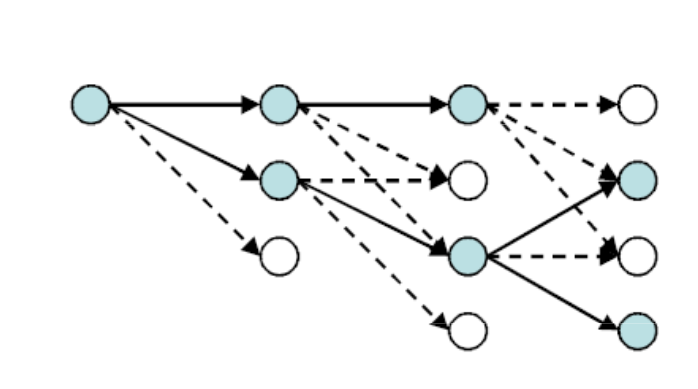
\includegraphics[width=6cm]{images/beam_search.png}
		\caption{Example of a beam search tree \cite{Beam:1}}
	\end{figure}

\end{frame}


\end{document}
